\documentclass{article}
\usepackage[utf8]{inputenc}
\usepackage{tikz,tcolorbox}
\usepackage{amsfonts, amsmath, amssymb, dsfont, amssymb,mathtools}
\usetikzlibrary{calc}

\title{RL2 - Markov Decision Process}
\author{sumit singh}
\date{\today}

\begin{document}

\maketitle

\section{Markov Processes}
\section{Markov Reward processes}
\subsection{Reward}
The \textit{return} $G_t$ is the total discounted reward from time-step $t$:
$$G_T = R_{t+1} + \gamma R_{t+2} + ... = \sum_{k=0}^{\infty} R_{t+k+1}   $$
\subsection{Value Function}
The \textit{state value function} $v(s)$ of an MRP is the expected return starting from state s:
$$v(s) = \mathbb{E}[G_t|S_t=s] $$
\subsection{Bellman Equation for MRPs}
The value function can be decomposed into two parts:
\begin{itemize}
    \item immediate reward $R_{t+1}$
    \item discounted value of successor state $\gamma v(S_{t+1})$
\end{itemize}
\begin{align*}
    v(s) &= \mathbb{E}[G_t|S_t=s]\\
         &= \mathbb{E}[R_{t+1} + \gamma R_{t+2} +\gamma^2 R_{t+3} + \cdots |S_t = s ] \\
         &= \mathbb{E}[R_{t+1} + \gamma(R_{t+2} + \gamma R_{t+3} + \cdots) | S_t =s] \\
         &= \mathbb{E}[R_{t+1} + \gamma G_{t+1} | S_t = s]\\
         &= \mathbb{E}[R_{t+1} + \gamma v(S_{t+1} | S_t= s ] \\
    v(s) &= R_s + \gamma \sum_{s' \in S} P_{SS'} v(s')
\end{align*}


\subsection{Bellman Equation in Matrix Form}
The Bellman equation can be expressed concisely using matrices,
$$ v = R + \gamma P v $$
where $v$ is a column vector with one entry per state
\begin{gather}
 \begin{bmatrix} v(1)  \\
                 \vdots  \\
                 v(n) 
 \end{bmatrix}
 =
  \begin{bmatrix} R(1)  \\
                 \vdots  \\
                 R(n) 
  \end{bmatrix}
+ \gamma 
  \begin{bmatrix}
   P_{11} & \dots &  P_{1n} \\
   \vdots & \ddots  & \vdots \\
   P_{11} & \dots & P_{nn}  
   \end{bmatrix}
    \begin{bmatrix} v(1)  \\
                 \vdots  \\
                 v(n) 
 \end{bmatrix}
\end{gather}
The Bellman equation is a linear equation and can be solved directly:
\begin{align*}
    v &= R + \gamma P v \\
    (1-\gamma P)v  &= R \\
    v &= (1-\gamma P)^{-1} R
\end{align*}
The computational complexity is $O(n^3)$ for $n$ states. Direct solutions only possible for small MRPs. There are many iterative methods for large MRPs, e.g.
\begin{itemize}
    \item Dynamic Programming
    \item Monte-Carlo evaluation
    \item Temporal Diffusion Learning 
\end{itemize}
%*********************************************************************************************************************
\section{Markov Decision Processes}
\subsection{Bellman Expectation Equation}
The state value function can be decomposed into immediate reward plus discounted value of successor state,
$$v_\pi(s) = \mathbb{E}[R_{t+1} + \gamma v_\pi (S_{t+1}) | S_t = s ] $$
The action-value function can similarly be decomposed:
$$  q_\pi (s,a) = \mathbb{E}_\pi [R_{t+1} + \gamma q_\pi (S_{t+1}, A_{t+1} | S_t=s, A_t = a]  $$
Bellman Expectation Equation for $v_\pi$:
$$v_\pi (s) = \sum_{a \in A}  \pi (a|s) q_\pi (s,a) $$
Bellman Expectation Equation for $Q^\pi$:
$$ q_\pi (s,a) = R_s^a + \gamma \sum_{s' \in S} P_{SS'}^a v_\pi (s')   $$
Bellman Expectation Equation for $v_\pi$:
$$v_\pi (s) = \sum_{a \in A}  \pi (a|s) ( R_s^a + \gamma \sum_{s' \in S} P_{ss'}^a v_\pi (s')  ) $$
Bellman Expectation Equation for $Q^\pi$:
$$ q_\pi (s,a) = R_s^a + \gamma \sum_{s' \in S} P_{SS'}^a \sum_{a \in A} \pi (a'|s') q_\pi (s',a')   $$
Bellman Expectation Equation (Matrix Form):
The Bellman expectation equation can be expressed concisely using the induced MRP,
$$v_\pi = R^\pi + \gamma P^\pi v_\pi$$
with direct solution
$$ v_\pi = (1 - \gamma P^\pi)^{-1} R^\pi $$

\subsection{Optimal Value Function}
The \textit{optimal state-value function} $v_* (s) $ is the maximum value function over all policies:
$$ v_*(s) = \underset{\pi}{\mathrm{max}}\, v_\pi (s) $$
The \textit{optimal action-value function} $q_* (s,a)$ is the maximum action-value function over all policies:
$$ q_* (s,a) = \underset{\pi}{\mathrm{max}}\  q_\pi (s,a) $$
The optimal value function specifies the best possible performance in the MDP. \\
An MDP is "solved" when we know the optimal value function. 

\subsection{Markov Decision Process}
A Markov Decision process is a Markov reward process with decisions. It is an \textit{environment} in which all states are Markov. \\
A \textit{Markov Decision Process} is a tuple  $(S,A,P,R, \gamma)$:
\begin{itemize}
    \item $S$ is a finite set of states
    \item $A$ is a finite set of actions
    \item $P$ is a state transition probability matrix,
    $$ P^a_{SS'} = \mathds{P}[S_{t+1} = s' | S_t = s, A_t = a]  $$
    \item $R$ is a reward function, $ R_s^a  = \mathbb{E}[R_{t+1} | S_t = s, A_t = a]     $
    \item $\gamma$ is a discount factor $\gamma \in [0,1]$

\end{itemize}
\subsection{Policies}
A $policy\ \pi $ is a distribution over action given states,
$$ \pi(a|s) = \mathds{P} [A_t=a | S_t =s]  $$
A policy fully defines the behavior of an agent. 

\subsection{Optimal Policy}
Define a partial ordering over policies

$$ \pi \geq \pi'\ \text{if}\ v_\pi (s) \geq v_{\pi'} (s), \forall s   $$
Theorem: \\
For any \textit{Markov Decision Process}:
\begin{itemize}
    \item There exists an optimal policy $\pi_*$ that is better than or equal to all other policies, $ \pi_* \geq \pi, \forall \pi $
    \item All optimal policies achieve the optimal value function, $v_{\pi_*}(s) = v_*(s)$
    \item All optimal policies achieve the optimal action-value function, $q_{\pi_*}(s,a) = q_*(s,a)  $
\end{itemize}
Finding an Optimal Policy:\\
An optimal policy can be found by maximising over $q_*(s,a)$,
\begin{equation}
  \pi_*(a|s) =
    \begin{cases}
      1 & \text{if  $a = \underset{a \in A}{\mathrm{argmax}}\, q_*(s,a) $}\\
      0 & \text{otherwise}
    \end{cases}       
\end{equation}
There is always a deterministic optimal policy for any MDP.\\
\subsection{Bellman Optimality Equation}
\subsubsection{Bellman Optimality Equation for $v_*$}
The optimal value functions are recursively related by the Bellman optimality equations:
$$ v_*(s) = \underset{a}{\mathrm{max}}\ q_*(s,a) $$
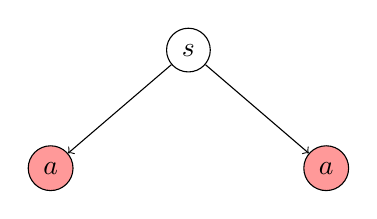
\begin{tikzpicture}[
    level distance=1.5cm,
    level 1/.style={sibling distance=3.5cm},
    level 2/.style={sibling distance=1cm}, ->]
    \tikzstyle{every node}=[circle,draw]
                
    \node (Root)  {$s$}
    child {
        node[fill=red!40] {$a$} 
    }
    child {
        node[fill=red!40] {$a$}
    }
    ;
\end{tikzpicture}
\subsubsection{Bellman Optimality Equation for $Q^*$}
$$ q_*(s,a) = R_s^a + \gamma \sum_{s' \in S} P_{SS'}^a v_*(s') $$
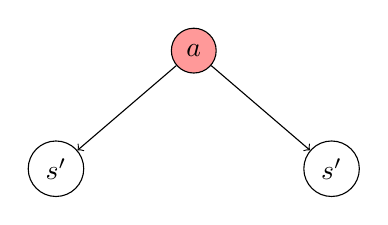
\begin{tikzpicture}[
    level distance=1.5cm,
    level 1/.style={sibling distance=3.5cm},
    level 2/.style={sibling distance=1cm}, ->]
    \tikzstyle{every node}=[circle,draw]
                
    \node (Root)[fill=red!40]  {$a$}
    child {
        node {$s'$} 
    }
    child {
        node {$s'$}
    }
    ;
\end{tikzpicture}
\subsubsection{Bellman Optimality Equation for $v_*$}
The optimal value functions are recursively related by the Bellman optimality equations:
$$ v_*(s) = \underset{a}{\mathrm{max}}\ R_s^a + \gamma \sum_{s' \in S} P_{SS'}^a v_* (s') $$
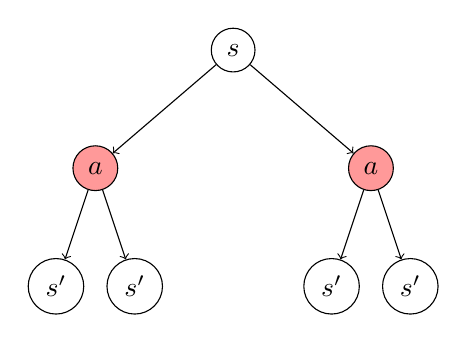
\begin{tikzpicture}[
    level distance=1.5cm,
    level 1/.style={sibling distance=3.5cm},
    level 2/.style={sibling distance=1cm}, ->]
    \tikzstyle{every node}=[circle,draw]
                
    \node (Root)  {$s$}
    child {
        node[fill=red!40] {$a$} 
        child { node {$s'$} }
        child { node {$s'$} }
    }
    child {
        node[fill=red!40] {$a$}
        child { node {$s'$} }
        child { node {$s'$} }
    }
    ;
\end{tikzpicture}
\subsubsection{Bellman Optimality Equation for $Q^*$}
$$ q_*(s,a) = R_s^a + \gamma \sum_{s' \in S} P_{SS'}^a \underset{a'}{\mathrm{max}}\ q_*(s',a') $$
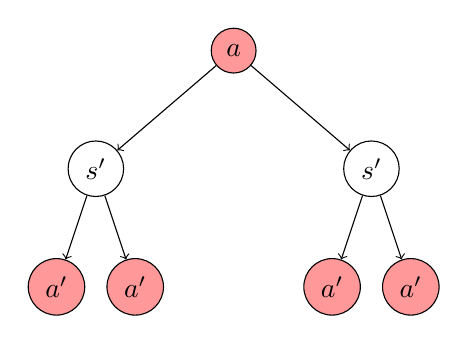
\begin{tikzpicture}[
    level distance=1.5cm,
    level 1/.style={sibling distance=3.5cm},
    level 2/.style={sibling distance=1cm}, ->]
    \tikzstyle{every node}=[circle,draw]
                
    \node (Root)[fill=red!40]  {$a$}
    child {
        node {$s'$} 
        child { node[fill=red!40] {$a'$} }
        child { node[fill=red!40] {$a'$} }
    }
    child {
        node {$s'$}
        child { node[fill=red!40] {$a'$} }
        child { node[fill=red!40] {$a'$} }
    }
    ;
\end{tikzpicture}

\subsubsection{Solving the Bellman Optimality equation}
\begin{itemize}
    \item Bellman Optimality Equation is non-linear
    \item No closed form solution (in general)
    \item Many iterative solution methods
    \begin{itemize}
        \item Value Iteration
        \item Policy Iteration
        \item Q-learning
        \item Sarsa
    \end{itemize}
\end{itemize}









\section{Extensions to MDP}
\section{Extensions to Dynamic Programming}
\section{Contraction Mapping}


\section{References}
$$
\[\underbrace{\text{New}Q(s,a)}_{\scriptstyle\text{New Q-Value}}=Q(s,a)+\mkern-34mu\underset{\text{New Q-Value}}{\underset{\Bigl|}{\alpha}}\mkern-30mu[\underbrace{R(s,a)}_{\scriptstyle\text{Reward}}+\mkern-30mu\underset{\text{Discount rate}}{\underset{\Biggl|}{\gamma}}\mkern-75mu\overbrace{\max Q'(s',a')}^{\scriptstyle\substack{\text{Maximum predicted reward, given} \\ \text{new state and all possible actions}}}\mkern-45mu-Q(s,a)]\]
$$
\begin{itemize}
    \item https://tex.stackexchange.com/questions/656416/how-to-circle-labels-below-tree-leaves-in-tikz
\end{itemize}

\end{document}